\chapter{Theorie der \glqq Mobile App Development Frameworks\grqq}

\section{Definitionen}

\subsection{Mobiles Endgerät}

Im weiteren Verlauf wird der Begriff mobile oder mobiles Endgerät in Anlehnung an das National Institute of Standards and Technology (NIST) genutzt. Diese definieren ein mobiles Endgerät als ein kleines Datenverarbeitungsgerät, welches leicht von einer einzelnen Person getragen werden kann. Dieses Mobile Gerät ist darauf ausgelegt ohne physische Verbindung zu funktionieren. Es besitzt einen lokalen, nicht entfernbaren Datenspeicher und wird über einen längeren Zeitraum von einer verbauten Energiequelle betrieben. Mobile Geräte können auch Sprachkommunikationsfähigkeiten, eingebaute Sensoren, die es dem Gerät ermöglichen, Informationen zu erfassen (z.B. Fotografie, Videoaufnahme und Standortbestimmung) und/oder eingebaute Funktionen zur Synchronisierung lokaler Daten mit weiteren Standorten enthalten\cite{nist1}.

\subsection{App/Applikation}

Mobile Apps werden im Folgenden auch als App bezeichnet. Der Begriff App ist innerhalb kürzester Zeit in den Sprachgebrauch eingegangen und wird weithin als eigenständige Anwendung auf einem mobilen Endgerät verstanden.
Apps werden von eigenständig dafür ausgelegten Plattformen heruntergeladen, welche von dem Hersteller des Betriebssystems zur Verfügung gestellt werden, oder direkt aus dem Internet bezogen.
Beispiele dafür sind der App Store bei iOS-Systemen und der Google Play Store bei Android-Systemen\cite{heikGrundl}.
\newpage
\subsection{Software-Framework}

Der Begriff Mobile App Framework ist nicht einheitlich definiert und kann je nach Kontext auf eine andere Art und Weise verwendet werden. Im Folgenden wird der Begriff Framework folgendermaßen definiert: \\

Bei einem Software-Framework handelt es sich um eine Abstraktion von Details, welche notwendig wären, um ein bestimmtes Ziel zu erreichen. Ein Framework stellt dem Entwickler eine gewisse Grundfunktionalität zur Verfügung, auf welcher aufgebaut werden kann, um eigene Software zu schreiben. Grundbausteine von Frameworks sind abstrakte oder konkrete Klassen, welche beerbt erweitert oder direkt verwendet werden können.\\

Frameworks lassen sich anhand der Kontrolle des Programmablaufes von einer Library abgrenzen. Während Frameworks die Kontrolle über den Programmablauf behalten und an bestimmten Stellen den vom Anwendungsentwickler eingefügten Code ausführen, stellen Librarys eine Ansammlung von Funktionen dar, welche vom Code des Anwendungsentwicklers aus aufgerufen werden können. Jedoch ist der Übergang von Framework zu Library fließend und hängt auch stark von dem Kontext ab in welchem der Begriff verwendet wird.\\

Martin Fowler definiert den Unterschied folgendermaßen:

\blockcquote{fowler1}{
	\glqq Inversion of Control is a key part of what makes a framework different to a library. A library is essentially a set of functions that you can call, these days usually organized into classes. Each call does some work and returns control to the client.
	A framework embodies some abstract design, with more behavior  built in. In order to use it you need to insert your behavior into various places in the framework either by subclassing or by plugging in your own classes. The framework's code then calls your code at these points.\grqq
}

\begin{figure}[h]
	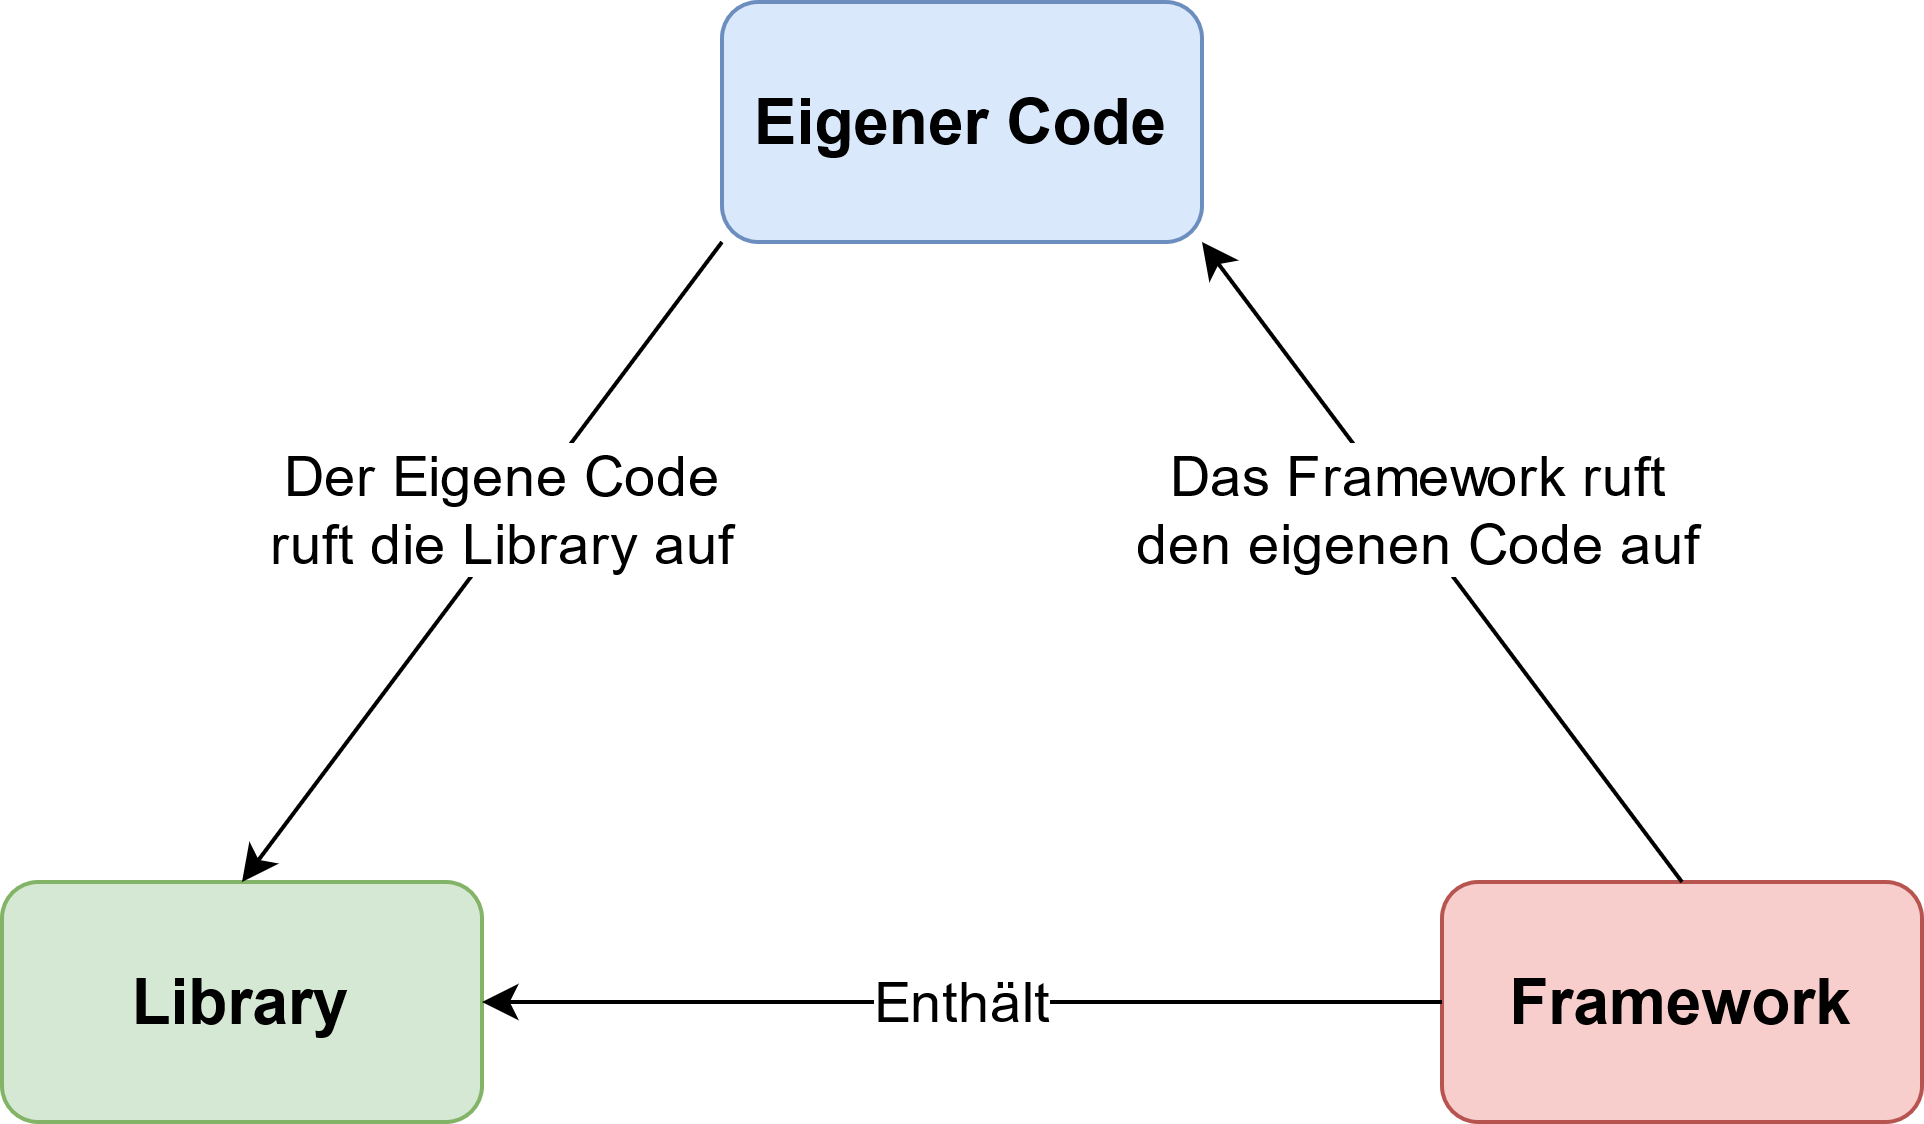
\includegraphics[scale=0.12]{frameworks}
	\centering
	\caption{Zusammenhang zwischen einer Library und einem Framework}
\end{figure}

\newpage

Zusätzlich zu der Unterscheidung zwischen Frameworks und Librarys existieren noch sogenannte \glqq opinionated\grqq\ und \glqq non-opinionated\grqq\ Frameworks bzw. Librarys. Bei opinionated Frameworks werden gewisse Vorgaben gemacht, z.B. wie die Ordnerstruktur des Projekts aussehen sollte oder wie gewisse Funktionen zu implementieren sind. Es wird ein Rahmen bereitgestellt, in welchem Beziehungen und Architektur der Komponenten vorgegeben werden. Abweichungen von diesem sind, je nachdem wie strikt diese durchgesetzt werden, schwer und nur mit viel Aufwand möglich. Non-opinionated Frameworks hingegen schreiben solch einen Rahmen nicht vor. Der Entwickler muss sich selber um bestimmte Aspekte wie z.B. den Anwendungszustand kümmern. Dies sorgt dafür, dass die Flexibilität auf Kosten der Komplexität erhöht wird\cite{opinionated}.\\

Ein Mobile Application Development Framework ist demnach ein Framework, welches die Struktur bereitstellt, eine Anwendung zu bauen, welche auf einem Mobilgerät ausgeführt werden soll.

\newpage
\section{Einsatzgebiete und Gründe für die Nutzung eines Mobile App Development Frameworks}

Die Gründe ein Framework in einem bestimmten Projekt zu nutzen sind sehr vielfältig und meist sehr individuell, da das Framework meist nur ein Hilfsmittel ist, um die Anforderungen an das Projekt zu erfüllen.\\

Bei Applikationen, dessen Zielgruppe Endbenutzer sind, besteht wie eingangs erwähnt die Notwendigkeit verschiedene Plattformen zu unterstützen, um eine größtmögliche Anzahl an Benutzern sicherzustellen. Dabei ist es finanziell und organisatorisch vorteilhaft nur eine einzige Codebasis pflegen zu müssen. Außerdem wird somit Feature, \ac{UX} und \ac{UI} Gleichheit sichergestellt.\cite{rieger_evaluation}\\

Die Herausforderung für mobile Endgeräte zu entwickeln, kommt nicht nur aus der Notwendigkeit für zwei unterschiedliche Plattformen mit verschiedenen Versionen zu entwickeln und diese über einen gewissen Zeitraum zu unterstützen, sondern auch durch die aufgesplitterte Android-Landschaft. Da Google Android als Betriebssystemplattform entwickelt, können Hersteller auf dieser aufbauend beliebige Modifikationen und Erweiterungen vornehmen\cite{andriod1}. Dies sorgt dafür, dass eine Vielzahl an unterschiedlichen Hard- und Softwarekombinationen existieren. Diese nutzen zwar alle Android als Plattform, das eigentliche Betriebssystem und die Hardware, auf der es läuft, unterscheiden sich trotzdem teilweise stark voneinander. 2015 gab es über 24.000 verschiedene Geräte, welche auf Android basierten von etwa 1.300 verschiedenen Herstellern\cite{opensignal1}.

\begin{figure}[h]
	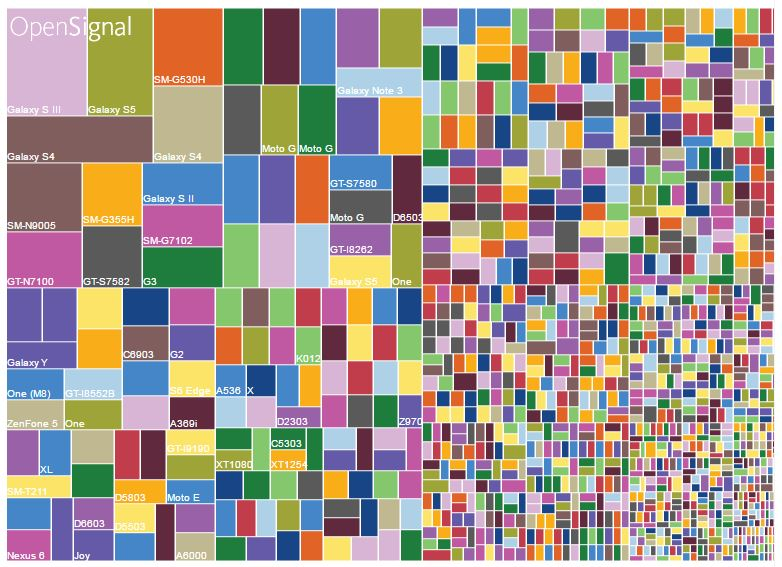
\includegraphics[scale=0.5]{androidfrag}
	\centering
	\caption[Visualisierung der Hardware-Fragmentierung von Android-Geräten]{Visualisierung der Hardware-Fragmentierung von Android-Geräten \cite{opensignal1}}
\end{figure}

\newpage
Hinzu kommt noch der Trend, dass immer mehr verschiedene Gerätetypen Android als Betriebssystem nutzen und dem User ebenfalls ermöglichen Apps auf diesen zu installieren. Zu den bereits bekannten Smartphones und Tablets sind in den letzten Jahren vermehrt Smartwatches, Autos und Smart TV Fernseher dazugekommen, welche ein Android-Basiertes Betriebssystem nutzen. Dies hat zur Folge, dass zusätzlich verschiedene Konnektivitätseigenschaften der Endgeräte berücksichtigt werden müssen. Zudem verschwimmen die Grenzen zwischen den Gerätetypen immer mehr. Jedes dieser verschiedenen Gerätetypen birgt Besonderheiten und Limitierungen, was die Entwicklung einer Anwendung, welche mit mehreren Typen kompatibel sein soll, teilweise stark verkomplizieren. Mit einigen der im Folgenden erwähnten Frameworks kann solch ein breites Spektrum an Endgeräten abgedeckt werden, jedoch wird im weiteren Verlauf der Arbeit näher darauf eingegangen, da diese Endgeräte teilweise der Definition von einem mobilen Endgerät nicht entsprechen und eine Berücksichtigung dieser den Rahmen sprengen würde.\\

Des Weiteren können Gründe für die Nutzung bestimmter Frameworks auch organisatorischer Natur sein und müssen nicht zwingend technisch begründet sein. Beispiele dafür können die Erfahrung und Größe des Entwicklungsteams, die Größe des Projekts, Vorgaben der Organisation, Lizenzen, verfügbares Budget und noch viele Weitere sein. Generell wird eine immer kürzere und effizientere Entwicklung von Software angestrebt, was eine Reduzierung von Entwicklungszeit und somit Kosten zur Folge hat. Diese Trend hat die Popularität der cross-plattform Entwicklung stark beeinflusst.

